%%%%%%%%%%%%%%%%%%%%%%%%%%%%%%%%%%%%%%%%%%%%%%%%%%%%%%%%%%%%%%%%%%%%%%%%
%% $Id$
%%%%%%%%%%%%%%%%%%%%%%%%%%%%%%%%%%%%%%%%%%%%%%%%%%%%%%%%%%%%%%%%%%%%%%%%
% This file and the files in this directory and its subdirectories
% are intended to test several parts of the TeXnicCenter-system.
%
% Copyright (C) 2002-$CurrentYear$ ToolsCenter

% Their main purpose is to reproduce several bugs or behaviours coming
% up from missing features. They are neither a good starting point for
% working with TeX nor with the TeXnicCenter-system. If you use them,
% you do this on your own risk. They come WITHOUT ANY WARRANTY;
% without even the implied warranty of MERCHANTABILITY or
% FITNESS FOR A PARTICULAR PURPOSE.
%
% Anything below the "end of prolog"-line is for testing purposes only
% and does not reflect the opinions of the author(s) and is not meant
% to be a statement at all; it is even not said to be true or reliable.
%
% If you have further questions or if you want to support
% further TeXnicCenter development, visit the TeXnicCenter-homepage
%
%     http://www.ToolsCenter.org
%
% end of prolog %%%%%%%%%%%%%%%%%%%%%%%%%%%%%%%%%%%%%%%%%%%%%%%%%%%%%%%%

% 25 Graphics

\begin{figure}
	\begin{center}
		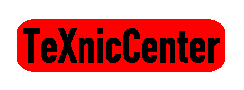
\includegraphics{txc.eps}
	\end{center}
	\caption{A Figure to stress the StructureParser}
\end{figure}

\begin{figure}
	\begin{center}
		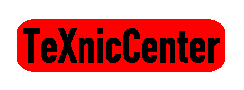
\includegraphics{txc.eps}
	\end{center}
	\caption{A Figure to stress the StructureParser}
\end{figure}

\begin{figure}
	\begin{center}
		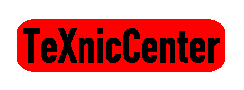
\includegraphics{txc.eps}
	\end{center}
	\caption{A Figure to stress the StructureParser}
\end{figure}

\begin{figure}
	\begin{center}
		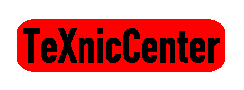
\includegraphics{txc.eps}
	\end{center}
	\caption{A Figure to stress the StructureParser}
\end{figure}

\begin{figure}
	\begin{center}
		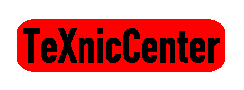
\includegraphics{txc.eps}
	\end{center}
	\caption{A Figure to stress the StructureParser}
\end{figure}


\clearpage


\begin{figure}
	\begin{center}
		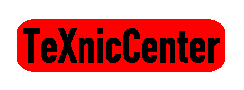
\includegraphics{txc.eps}
	\end{center}
	\caption{A Figure to stress the StructureParser}
\end{figure}

\begin{figure}
	\begin{center}
		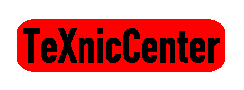
\includegraphics{txc.eps}
	\end{center}
	\caption{A Figure to stress the StructureParser}
\end{figure}

\begin{figure}
	\begin{center}
		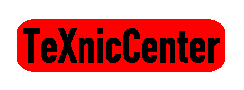
\includegraphics{txc.eps}
	\end{center}
	\caption{A Figure to stress the StructureParser}
\end{figure}

\begin{figure}
	\begin{center}
		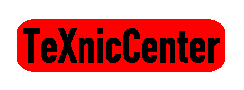
\includegraphics{txc.eps}
	\end{center}
	\caption{A Figure to stress the StructureParser}
\end{figure}

\begin{figure}
	\begin{center}
		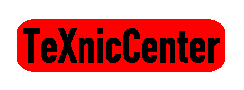
\includegraphics{txc.eps}
	\end{center}
	\caption{A Figure to stress the StructureParser}
\end{figure}


\clearpage


\begin{figure}
	\begin{center}
		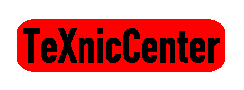
\includegraphics{txc.eps}
	\end{center}
	\caption{A Figure to stress the StructureParser}
\end{figure}

\begin{figure}
	\begin{center}
		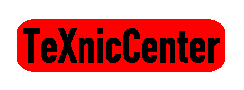
\includegraphics{txc.eps}
	\end{center}
	\caption{A Figure to stress the StructureParser}
\end{figure}

\begin{figure}
	\begin{center}
		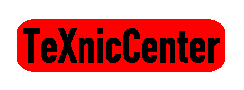
\includegraphics{txc.eps}
	\end{center}
	\caption{A Figure to stress the StructureParser}
\end{figure}

\begin{figure}
	\begin{center}
		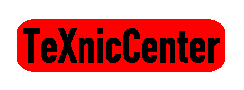
\includegraphics{txc.eps}
	\end{center}
	\caption{A Figure to stress the StructureParser}
\end{figure}

\begin{figure}
	\begin{center}
		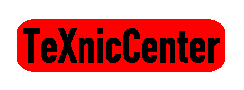
\includegraphics{txc.eps}
	\end{center}
	\caption{A Figure to stress the StructureParser}
\end{figure}


\clearpage


\begin{figure}
	\begin{center}
		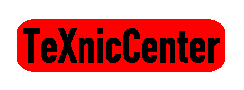
\includegraphics{txc.eps}
	\end{center}
	\caption{A Figure to stress the StructureParser}
\end{figure}

\begin{figure}
	\begin{center}
		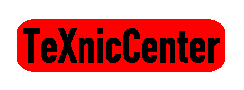
\includegraphics{txc.eps}
	\end{center}
	\caption{A Figure to stress the StructureParser}
\end{figure}

\begin{figure}
	\begin{center}
		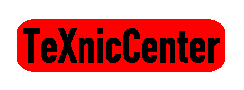
\includegraphics{txc.eps}
	\end{center}
	\caption{A Figure to stress the StructureParser}
\end{figure}

\begin{figure}
	\begin{center}
		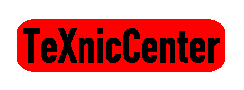
\includegraphics{txc.eps}
	\end{center}
	\caption{A Figure to stress the StructureParser}
\end{figure}

\begin{figure}
	\begin{center}
		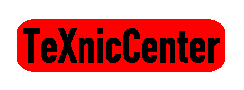
\includegraphics{txc.eps}
	\end{center}
	\caption{A Figure to stress the StructureParser}
\end{figure}


\clearpage

\begin{figure}
	\begin{center}
		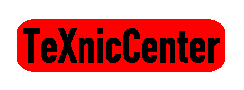
\includegraphics{txc.eps}
	\end{center}
	\caption{A Figure to stress the StructureParser}
\end{figure}

\begin{figure}
	\begin{center}
		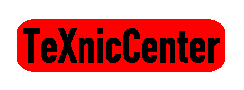
\includegraphics{txc.eps}
	\end{center}
	\caption{A Figure to stress the StructureParser}
\end{figure}

\begin{figure}
	\begin{center}
		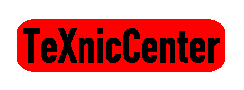
\includegraphics{txc.eps}
	\end{center}
	\caption{A Figure to stress the StructureParser}
\end{figure}

\begin{figure}
	\begin{center}
		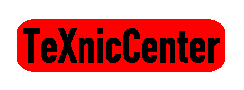
\includegraphics{txc.eps}
	\end{center}
	\caption{A Figure to stress the StructureParser}
\end{figure}

\begin{figure}
	\begin{center}
		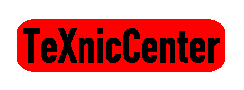
\includegraphics{txc.eps}
	\end{center}
	\caption{A Figure to stress the StructureParser}
\end{figure}


\clearpage

